\documentclass[10pt]{article}
\title{ Topology as a Tool to Differentiate Canopy Architecture in North American Forests }
\author{ Eva Arroyo, Samuel Pease, Nikita Zemlevskiy}
\date{5/4/2017}
\usepackage{graphicx}
\begin{document}
\maketitle
\newpage
\section*{Introduction}

\indent Canopy architecture describes the surface of the tops of trees in a forest, how they overlay and grow over each other, how high they are, and what the shape of each individual tree is. Canopy architecture reflects disturbance history and species composition. These can be related to biomass, light availability, and disturbance (1).  The competition for light requires different species to niche differentiate and optimize for different amounts of light. In forests with high diversity of trees, there will (CITE) likely be high niche differentiation on all scales in order to live concurrently in the same forest. This will therefore be reflected in the canopy architecture, with more layers to the canopy. A mystery that has long puzzled ecologists is on the diversity of the tropical rainforest, and how so many species are able to live in the same forest (SEE IF YOU CAN RELATE THIS TO CANOPY ARCH OTHERWISE REMOVE). In addition, canopy architecture reflects disturbance history. If a canopy is disturbed in a significant way, such as through wind damage, this will likely cause tree toppling, which then creates a hole in the canopy. Though this hole will regrow, filled with other plants, the long term effects will be seen in the canopy architecture for up to 65 years afterwords (1). Disturbance history has profound effects on biomass, often secondary growth can result in a high net carbon sink, though decomposition will inevitably reverse this trend. In addition, anthropogenic changes can act as a large scale disturbance, which can similarly differentiate logged and unlogged forests for many years after the disturbance event. Canopy architecture is one of the summaries we have of complex forested ecosystems, and summarizing forest structure in a meaningful way can lead to understanding of how niche differentiation affects the whole forest.

\indent The advent of LiDAR has allowed ecologists to remotely examine forest canopy heights . LiDAR functions by sending a burst of infrared light and recording the time it takes for light to return to the source, then using this to determine the distance the source is away from the detector. They can take several hundred samples in less than a second, making them extremely effective (CITE) By using this technology in planes flying over land surface, ecologists can obtain a very precise visualization of the canopy height across a forest, improving previous methods of assessing forest structure and size from ground transects. However, many methods using LiDAR are unable to make use of the topological data, simplifying it into maximum height and canopy size distribution across a forest, reducing data on a surface to data on a point. Persistence diagrams as a way of measuring both height and evenness, therefore have the potential to describe this surface of the canopy without reduction. Here we use four parks from the United States, to examine if persistence diagrams from LiDAR data can differentiate the different parks, and if these ecologically diverse sites with different disturbance regimes have significantly different canopy structure as analyzed with topological methods. We do not seek necessarily to explain differences in persistence across these forests, but to establish that persistence can differentiate these forests which should theoretically have vastly different canopy structures.


\section*{Data}
\indent We obtained LiDAR data from the National Ecological Observatory Network. The LiDAR dataset included interpretations of the raw waveform and point based returns into models of canopy height (CHMs), with just one tree height per pixel, which was what we used for our analyses. From the larger dataset of 13 ecological regions we imported LiDAR data from four sites Bartlett (BART), Great Smoky Mountains (GRSM), Harvard Forest (HARV), and Mountain Lake Biological Station (MLBS) from the Northeastern and Appalachian ecological regions on the eastern coast of the United States. These forests have significantly different forest structures and disturbance histories, from Harvard Forest, is a Northeastern experimental forest that has been selectively logged (CITE site); Mountain Lake Biological station, a forest in the Appalachian mountains of Virginia with history of chestnut blights (2); Great Smoky Mountains National Park, with a history of logging in the 1800s; and Bartlett forest which has selective logging. In addition these sites have vastly different species compositions, due to differences in soils and elevations, so we predict differences in canopy structure over all sites. These collectively resulted in 1050 CHMs upon which we ran our analyses.

\section*{Topological Methods}
\indent To perform topological analysis and extract persistence diagrams from the data, two methods were used. The first of these methods was to obtain transects from the forest data. Transects are the canopy heights in one line across one a forest, creating a function along a line of canopy heights.These functions of one variable that mapped from x coordinate to height at that coordinate on the respective transect were generated for a random line across each CHM for each forest. Next, a standard sublevel-set filtration was performed on the function to create persistence diagrams. Zero dimensional persistence diagrams were obtained as a result of this method. Since the data was two dimensional by nature, we were interested how this method would compare to a 2 dimensional case, which led us to our second method.\\

\indent The second method of obtaining persistence diagrams was to consider the data to be a function of two variables. For this we overlaid a grid over the forest and at each coordinate the function was equal to the height of the canopy there. Next, we took a 2 dimensional sublevel-set filtration of the function. By sweeping from the minimum height to the maximum height, we were able to obtain persistence diagrams for the data. To accomplish this task, we used the code written by Dr. Nate Strawn provided by Dr. Chris Tralie. Using this method, zero and one dimensional persistence diagrams of this representation of the data were obtained. Once we had generated persistence diagrams from all of our data we converted them into graphs of persistence plotted against birthtime. We summarize the persistence diagrams for each site by reporting the maximum persistence across all CHMs, the mean maximum persistence for each persistence diagram in the data set for the site, and the mean of the mean persistence for each persistence diagram in each site.

\section*{Machine Learning Methods}

\indent From the persistence diagrams, we overlaid a grid and counted the number of points that fell within each grid cell in order to generate vectors. For each type of persistence we first found the longest persistence across all diagrams and use this as the maximum value for all grids in order to generate equal-length vectors. The grids went from zero to this maximum value by ones.

\indent Next we used these high dimensional vectors to do machine learning through SVM. SVM learning or support vector machine learning is a process of finding the hyperplane that best separates data points by category. However there are many examples of data that is clearly separable but not simply by a hyperplane, such as data easily separated by a circle. In these cases a kernel function is used. This is done by raising the dimension of the data so that a hyperplane does accurately separate the categories of data. In order to determine which kernel was the most effective at separating data we used cross validation. The data was split up into training ($80\%$ of the data in all cases) and validation data so that we could test our classification on different vectors than those used to generate the separating hyper plane. The classification was then tested on the testing data using the different kernel functions and different cost and gamma values as the parameters of the classification. The optimal kernel function, cast, and gamma values were then selected to produce a hyperplane that best separated the data by category. To do this we used code from Deepanshu Bhalla.

\indent We ran the SVM to classify all four of our forests. This classifies each of the four variables against every other variable and then using a voting technique to achieve the best overall prediction model. We report all sites with Kolmogorov-Smirnof (KS) tests for goodness of fit of our SVMs, and area under the receiver operating curves for accuracy of prediction.

\section*{Results}
\subsection*{Transects}

We calculated transect data for four sites and a total of 224 persistence diagrams. Across sites, seven had to be removed, which resulted in blank persistence diagrams. The highest persistence is for the Great Smoky Mountains as well as the highest mean maximum persistence (Table 1). The calculated area under the curve was 0.610 (Figure 1), and a KS of 0.242.\\


\begin{table}[]
\centering
\caption{Summary statistics across all transects in a specific site with mean and standard deviation in parenthesis.}
\begin{tabular}{|l|l|l|l|l|}
\hline
                         & BART          & GRSM          & HARV          & MLBS          \\ \hline
Mean Maximum Persistence & 22.18 (2.907) & 29.75 (6.845) & 23.21 (3.141) & 24.71 (5.240) \\ \hline
Maximum Persistence      & 31            & 49            & 38            & 39            \\ \hline
Mean Mean Persistence    & 7.610 (1.799) & 8.453 (2.005) & 5.869 (3.090) & 7.156 (2.452) \\ \hline
\end{tabular}
\end{table}


\noindent 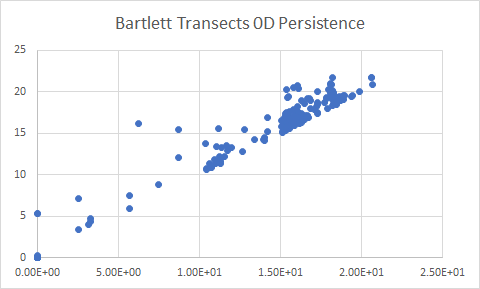
\includegraphics[scale = 0.5]{bartlett_transects_0d_persistence}
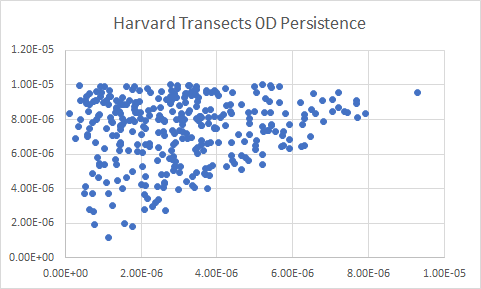
\includegraphics[scale = 0.5]{harvard_transects_0d_persistence}
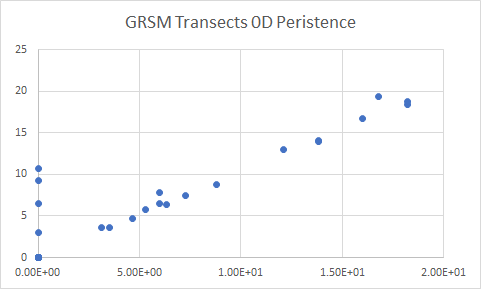
\includegraphics[scale = 0.5]{grsm_transects_0d_persistence}
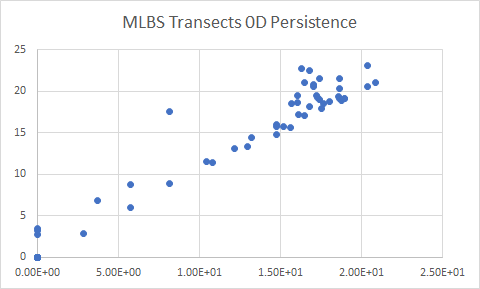
\includegraphics[scale = 0.5]{mlbs_transects_0d_persistence}\\
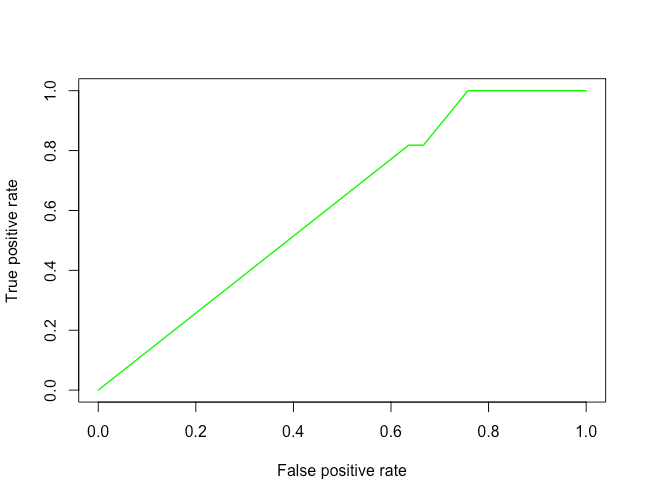
\includegraphics[scale = 0.5]{transect_roc}\\
Figure 1: False positives versus true positives for prediction of site 1 using the transect method


\subsection*{0 Dimensional Persistence}

We analysed a total of 400 canopy height models over the four sites to examine the zero dimensional persistence. The highest average maximum persistence was at the Great Smoky Mountains Part, though the highest single value was at Bartlett forest (Table 2). This resulted in an AUC of .544 and a KS of .088 (Figure 2).\\

\noindent 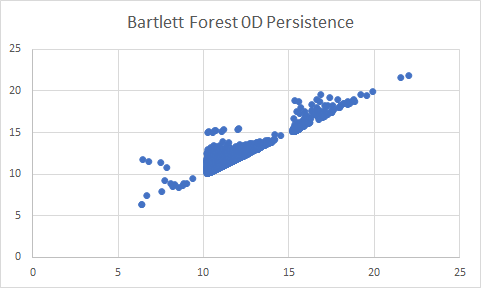
\includegraphics[scale= 0.5]{bartlett_0d_persistence}
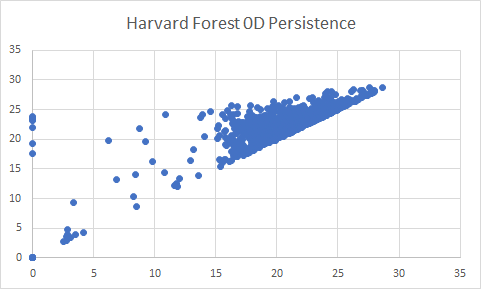
\includegraphics[scale= 0.5]{harvard_0d_persistence}
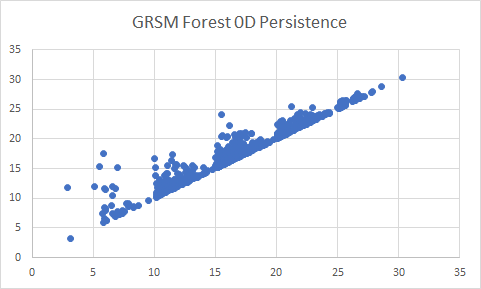
\includegraphics[scale= 0.5]{grsm_0d_persistence}
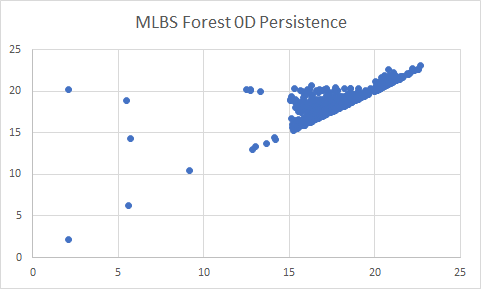
\includegraphics[scale= 0.5]{mlbs_0d_persistence}\\
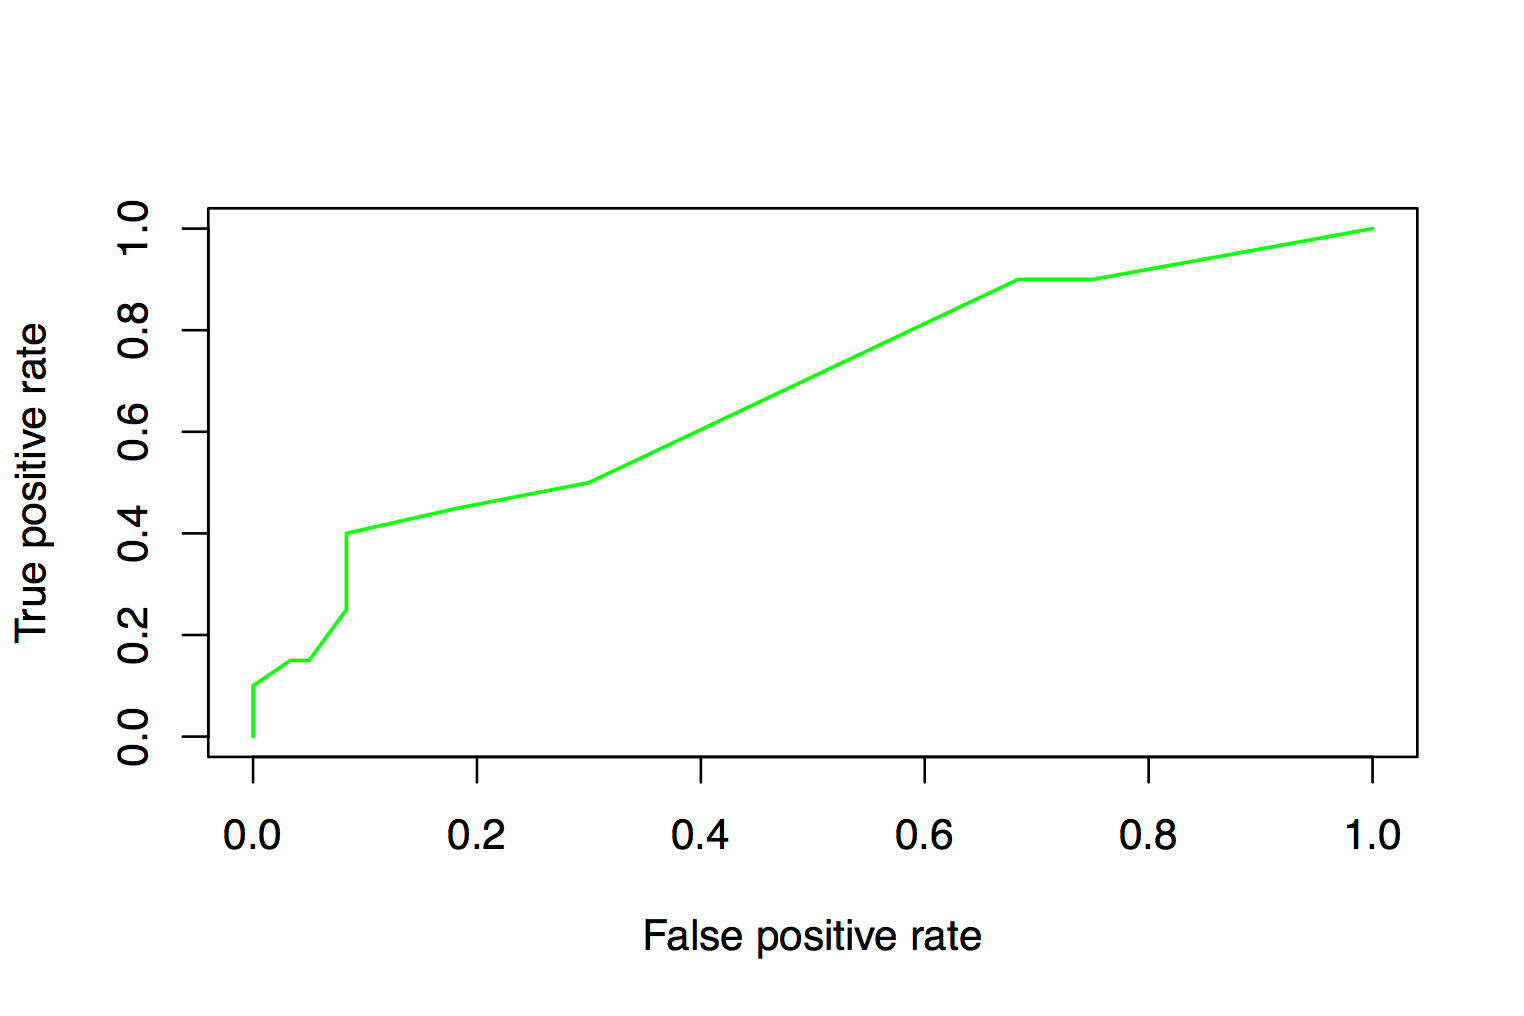
\includegraphics[scale= 0.5]{0d_roc}\\
Figure 2: True positive by false positives for the 0D persistence of the Canopy Height Models

\begin{table}[]
\centering
\caption{Summary statistics across all data in a specific site with mean and standard deviation in brackets}
\begin{tabular}{|l|l|l|l|l|}
\hline
                         & BART          & GRSM          & HARV          & MLBS          \\ \hline
Mean Maximum Persistence & 16.19,(1.375) & 24.991,(2.844) & 21.725,(3.361) & 22.693,(2.703)  \\ \hline
Maximum Persistence      &50            & 27            & 31            & 31            \\ \hline
Mean Mean Persistence    & 3.604,(.906) & 4.473,(1.571) & 5.133,(1.926) & 5.314,(1.784) \\ \hline
\end{tabular}
\end{table}

\subsection*{1 Dimensional Persistance}
We used the same set of 400 canopy height models for the one dimensional persistencehis resulted in a AUC of .709 and a KS of .37 (Figure 3). The highest average maximum persistence across sites was at GRSM, MLBS had the highest mean mean persistence, and BART had the highest overall persistence (Table 3).\\
\noindent 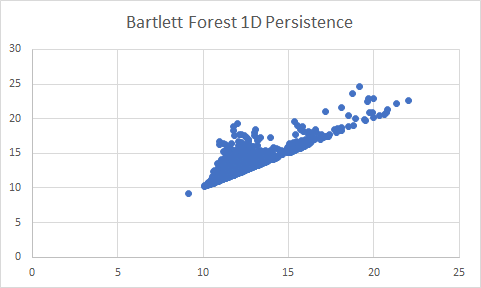
\includegraphics[scale= 0.5]{bartlett_1d}
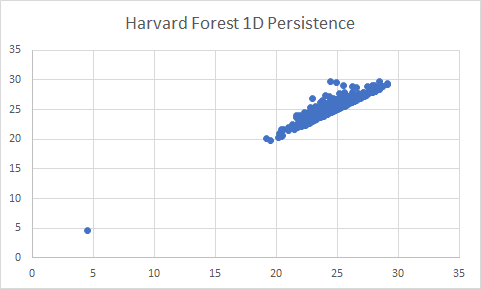
\includegraphics[scale= 0.5]{harvard_1d}
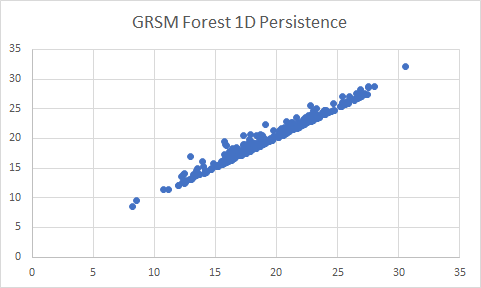
\includegraphics[scale= 0.5]{grsm_1d}
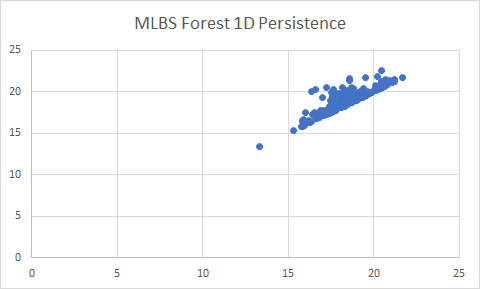
\includegraphics[scale= 0.5]{mlbs_1d}\\
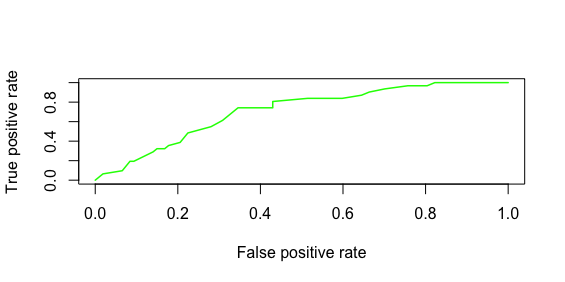
\includegraphics[scale= 0.5]{1d_roc}\\
Figure 3: True positive by false positives for the 1-D persistence of the Canopy Height Models

\begin{table}[]
\centering
\caption{Summary statistics across all data at a specific site with mean and standard deviation in brackets}
\begin{tabular}{|l|l|l|l|l|}
\hline
                         & BART          & GRSM           & HARV          & MLBS          \\ \hline
Mean Maximum Persistence & 16.19,(1.375) & 24.991,(3.528)  & 21.725,(3.361) & 22,693,(2.703) \\ \hline
Maximum Persistence      & 50            & 27             & 31            & 31            \\ \hline
Mean Mean Persistence    & 3.604,(.906) & 4.473,(1.571) & 5.133,(1.926) & 5.314,(1.784) \\ \hline
\end{tabular}
\end{table}


\section*{Discussion}
\indent The SVMs were considerably more effective at classifying feature vectors constructed from 1d persistence diagrams than the other two methods, the transect 0d method and the non-transect 0d method. Running the classification on 1d persistence diagrams, an AUC value of 0.815 was obtained, compared to 0.61 and 0.67 for the transect and non transect 0d methods respectfully. Since a higher AUC corresponds to a higher correct classification rate, our results indicate that the 1d methodology is better for classifying persistence diagrams of canopy height models. 

\indent We interpret 0d persistence (for both the transect and the non-transect cases) as the heights of individual trees relative to those around it. This is analogous to sampling a function where each point is a tree, and persistence comes from comparing heights of points to heights of their neighbors. In contrast, 1d persistence is a measure of more general trend-like increases. Such an increase could be caused by a mountain or hill, since the elevations would be getting higher and higher and would reach a maximum at the middle. Although ground level elevation is accounted for in the model and only height from the ground is provided in the data, the analogy is still useful. One could imagine a group of trees that get gradually taller and taller closer to the middle of the group. 1d persistence measures the size and importance of such groups. As such, these are two fundamentally different but related quantities, and it is acceptable that results from using them could vary.

\indent Taking a closer look at the 0d transect data, we can see that the persistence diagrams look quite similar. In particular, diagrams from all the considered sites except for the Harvard site look somewhat alike, with many points close to the diagonal. The The Harvard diagram is interesting to think about, in that the diagram is quite spread out. There are many persistence points with early birth and late death. This must have been an important distinguishing factor in classifying the profiles forests. However, the similarity of the other 3 forest sites must have made the classification process less effective. The same could be said for the 0d non-transect method. These diagrams are less similar, however, than the ones from the transect data. Despite this fact, this method still did not do as well as the 1d method. In this case, there were two pairs of similar diagrams, Bartlett and GRSM, and MLBS and Harvard. It is interesting to note that the persistence diagram of the Harvard site resembles that of the transect data, which makes intuitive sense.

\indent Although the diagrams for the MLBS and Harvard sites for 1d persistence look similar in that both of them have a lot of points high up on or near the diagonal, the 1d method still gave a better classification model. A logical conclusion from this may be that forests are better identified not by how big the differences between individual trees are, but how many uniform trends there are, in terms of height. In other words, it is easier to classify a forest based on groups of tall trees and groups of short trees, getting taller and shorter in the middle of the group. This may have more biologically sophisticated explanations, but individual trees (0d persistence) may be accidents, while group-like trends (1d persistence) are harder to come upon accidentally. Sometimes a tall tree in a usually short forest survives, but many don't due to various environmental factors.

\indent The data resource that was used in this study contained immense amounts of data. This study could be extended to any number of forest locations, following a similar methodology that was outlined in this study. The data resource also contains numerous other attributes measured across the forests, not just canopy height information. Examples of these attributes include soil type information, logging information and other information. Including variables such as those into the classification model could prove beneficial, and may create a better predictor. In addition, it would be useful to classify on these additional parameters, not just on forest type/location. Such a model could be useful for various reasons. One may be interested in finding out whether a forest was logged or not, or what kind of soil a forest most likely has without actually sampling the forest. This would be possible from these additional models. Other classification methods, such as k nearest nearest neighbors may prove to be more effective, and a logical extension of this study would be to compare the performance of different learning methods.

\section*{Bibliography}
Bhalla, D. (2017 ). Support Vector Machine Simplified using R. Retrieved May 02, 2017, from http://www.listendata.com/2017/01/support-vector-machine-in-r-tutorial.html
Strawn, N. (n.d.). MORSEFILTRATION2D. Retrieved from https://d1b10bmlvqabco.cloudfront.net/attach/j1m8suensxh6ez/ho32xurye2y7nv/j1o35t5rkuhu/morseFiltration2D.m.

\end{document}
